%!TEX root = ../main_article.tex

\section{Related Work}

Our work is related to the following two fields: 

\subsection{Code Search}

Recent years’ works adopt deep learning models in code search, of which the idea is to embed natural language queries and program code into vectors and then calculate their similarity score. 
Fig~\ref{fig:cs_frame} shows the framework of code search: a code encoder, a natural language encoder, and a similarity calculator. The encoder transforms code or queries into high-dimensional vectors, which are considered semantic information. The calculator o computes the similarity between the two vectors. 

\begin{figure}[htb]
	\centering
	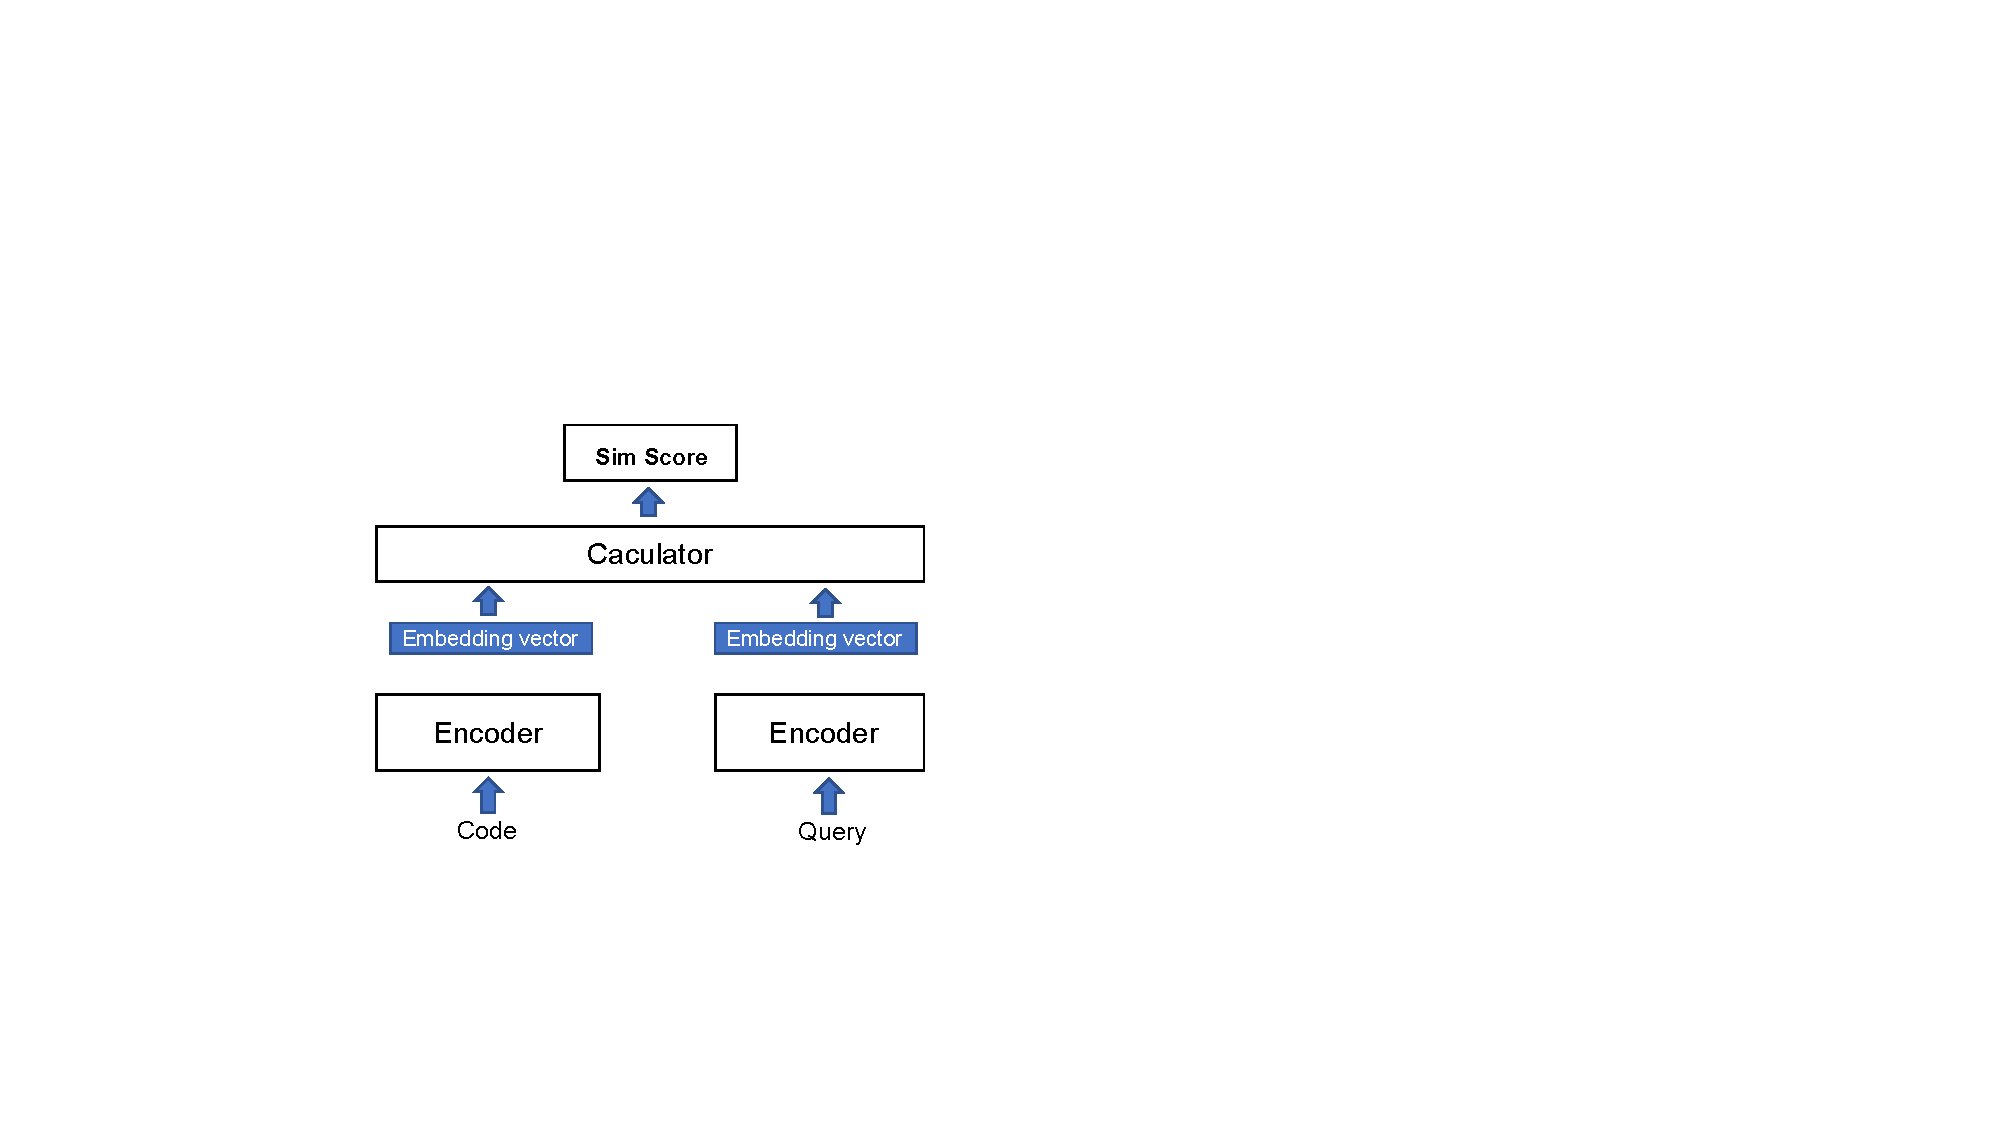
\includegraphics[width=0.8\linewidth]{imgs/code_search_framework.pdf}
	% \vspace{-15pt}
	\caption{Structure of the search enhancement framework.}
	% \vspace{-12pt}
	\label{fig:cs_frame}
\end{figure}

Models in code search based on deep learning can be roughly 
divided into the following aspects:

(1) RNN based models. Gu et al. (\citealp{DeepCS})
build two networks to embed queries and program code into vectors, respectively. 
Cosine similarity is used to compute the similarity between the vectors. 

(2) CNNs based models. Followed by (\citealp{DeepCS}), Li et al. (\citealp{CQIL}) construct “name-query” 
and “body-query” latex match matrix with fastText (\citealp{fastText}) and use 
CNNs to extract features.  

(3) PLMs. Feng et al. (\citealp{CodeBERT}) followed the idea of BERT (\citealp{BERT}) 
and proposed a pre-train model training on CSN (\citealp{CodeSearchNet}) 
dataset with hybrid objective functions: MLM (Masked Language Modeling) 
and RTD (Replaced Token Detection). (\citealp{GraphCodeBERT}) leverage data flow to 
enhance code representation. 
For the code data flow, they specifically designed a series of pre-training tasks: 
MLM, Edge Prediction, and Node Alignment. (\citealp{UniXcoder}) 
tranfrom code AST (Abstract Syntex Tree) to a sequence structure, 
thus the pre-training can utilize multi-modal contents. 


% In this section, we introduce existing code search methods and machine learning debiasing methods. 
% code search methods

% Our work is closely related to the following two domains:

% \vspace{3pt}
% \noindent\textbf{Code Search.} There is a tremendous amount of research on code search. 
% Early works adopt traditional information retrieval methods like Boolean Model~\cite{SaltonFW83}, Vector Space Model~\cite{SaltonWY75} 
% and Structural Semantic Indexing~\citep{Dumais04} to estimate 
% the relevance between the query and a code snippet~\citep{LvZLWZZ15,BajracharyaOL10}.
% Recent works adopt deep neural networks to embed query and code into vectors.
% Then, the code search task is performed by measuring the similarity 
% (e.g., cosine similarity) between vectors.
% % \yl{some are bi-encoder architecture, as described here, but many are cross-encoder architecture such as CodeBERT. Should describe them separately.}
% Along this direction, various deep learning based code search methods have been proposed, 
% including but not limited to 
% recurrent neural network (RNN) based approaches~\citep{DeepCS}, 
% convolutional neural network (CNN) based approaches~\citep{CQIL, ShuaiX0Y0L20}, 
% graph neural network (GNN) based approaches~\citep{WanSSXZ0Y19}
% and pre-training approaches~\citep{CodeBERT, GraphCodeBERT, GuoLDW0022}.


% \subsection{Code Search}
% In this section, we introduce existing code search methods and machine learning debiasing methods. 

% The challenge of code search is to effectively measure the 
% semantic similarity between natural language queries and program code. 
% More specifically, it is to find the semantically best matching 
% answer from several candidate codes when facing query statements 
% entered by developers. Code search methods can be divided into two categories: 
% information retrieval based models and deep learning based models. 
% The former is usually based on keyword matching. 

% Researchers have proposed code search models with diverse network architecture: 
% (1) RNN based models (\citep{DeepCS}). (2) CNN based models (\citep{CQIL, ShuaiX0Y0L20}). (3) PLMs (\citep{CodeBERT, CoCLR, GuoLDW0022}). 
% (4) Graph based models (\citep{GraphCodeBERT, GuCM21}).
% In all of them, the core idea is to measure the similarity between queries and code. 
% Common to these approaches is the conversion of queries and 
% codes into high-dimensional embedding vectors.

\subsection{Generative Adversarial Nets}
Adversarial training is an effective approach to enhance the robustness of a deep learning model(\citealp{bai2021recent}). And generative models are able to learn the probability distribution that generated the training examples. Generative adversarial networks(GANs) then performs well in generating more examples from the estimated probability distribution(\citealp{goodfellow2020generative}) so that it becomes a hot research topic recently.

Generally, GAN(\citealp{10.5555/2969033.2969125}) is similar to a minimax two-player game: one is a generative model $G$ that captures the data distribution, and the other player is a discriminative model $D$ that estimates the probability that an example came from the training data rather than $G$, i.e. to determine whether an example is from the model distribution or the data distribution. Both $G$ and $D$ are defined by multilayer perceptrons and are trained simultaneously. Competitions among these two players drives both to improve their performance respectively. And the value function in this game can be referred to as
\begin{equation}
\begin{split}
\mathop{min}\limits_{G}\mathop{max}\limits_{D}V(D,G)&=E_{x\sim p_{data}(x)}[log D(x)]\\ &+E_{z\sim p_{z}(z)}[log (1-D(G(z)))]
\end{split}
\end{equation}
where $p_{data}(x)$ is the distribution over data $x$, $z$ is the input noise, $G(z)$ represents a mapping from $z$ to data space, and $D(x)$ refers to the probability that $x$ came from the data rather than $G$.

In practice, the GANs must be implemented using an iterative, numerical approach, i.e. alternating between $k$ steps of optimizing $D$ and one step of optimizing $G$. And finally the training or the game terminates at a saddle point that is a minimum with respect to one player's strategy and a maximum with respect to the other player's strategy.

